\section{Movielens set ratings dataset} \label{ch:lfs:dataset}
\subsection{Data collection}
\ML is a recommender system that utilizes
collaborative filtering algorithms to recommend movies to their users based on
their preferences. We developed a set rating widget to obtain ratings on a set
of movies from the \ML users.  
The set rating widget could be
rated from 0.5 to 5 with a precision of 0.5.  
For the purpose of data collection, we selected users who were active since
January 2015 and have rated at least 25 movies. The selected users were
encouraged to participate by contacting them via email. 
The sets of movies that we asked a user to rate were created by selecting five
movies at random without replacement from the movies that they have already
rated. Furthermore, we limited the number of
sets a user can rate in a session to 50, though users can potentially rate
more sets in different sessions.
The set rating widget went live on February 2016 and, for the purpose of this
study, we used the set ratings that were provided until April 2016.



\begin{figure}[ht]
  \centerline{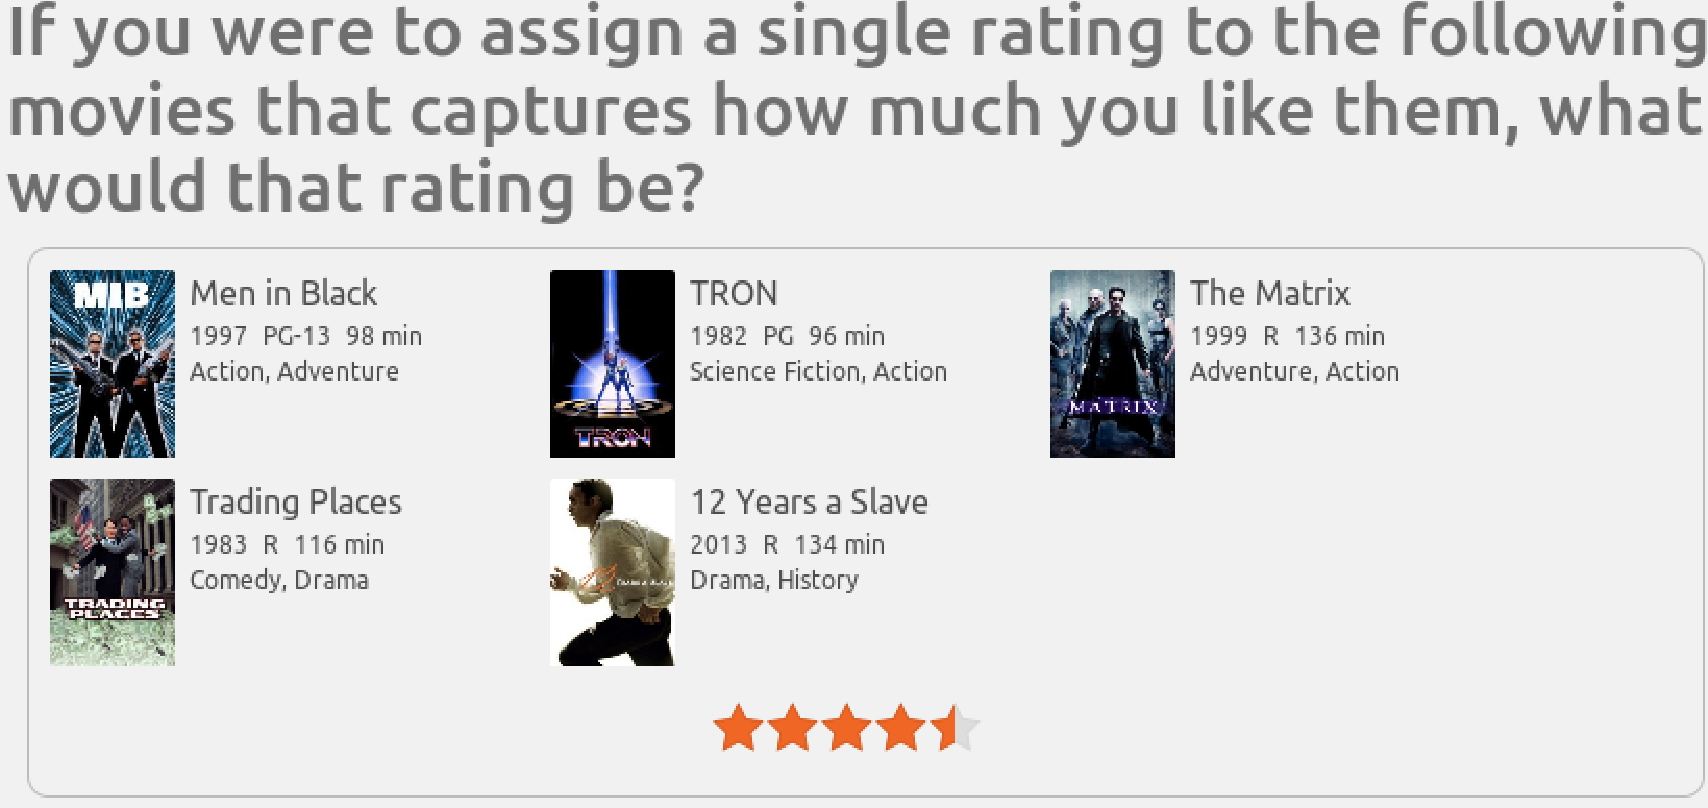
\includegraphics[scale=0.28]{figures/mlset.pdf}}
  \caption{The interface used to elicit users' ratings on a set of movies.}
  \label{fig:mlset}
\end{figure}

\subsection {Data processing}
From the initially collected data, we removed users who have rated sets within a
time interval of less than one second to avoid users who might be providing
the ratings at random. After this pre-processing, we were left with ratings
from 854 users over 29,516  sets containing 12,549 movies.
Figure~\ref{fig:usersetdist} 
shows the distribution of the number of sets rated by the users,
which shows that roughly half of the users have rated at least 45 sets in a session.


\begin{figure}[bt]
  \centerline{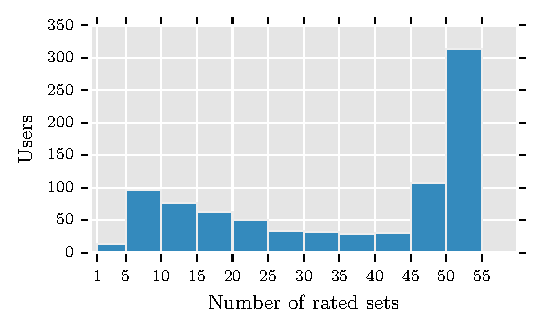
\includegraphics[scale=0.9]{figures/usersetdist.pdf}}
  \caption{The distribution of number of sets rated by the users.}
  \label{fig:usersetdist}
\end{figure}


\subsection{Analysis of the set ratings}\label{ch:lfs:data_analysis}

We investigated whether ratings are distributed uniformly or if some ratings
tend to appear more than others.
Figure~\ref{fig:itemsetratingdist} (left) depicts
the distribution of the collected ratings over all the sets. 
The majority of the ratings lie between 3.0 and 4.0. 
Since, by construction, we know the actual ratings that these users provided on
the actual movies. Figure~\ref{fig:itemsetratingdist} (right) shows the
distribution of the ratings of the movies that were contained in all these sets.
By comparing these distributions we can see that the average item-rating (3.50) is
somewhat higher than the average set-based rating (3.44) but the overall variance of
the set-based ratings (0.65) is lower than that of the item ratings (1.01).

\begin{figure}[t]
  \centerline{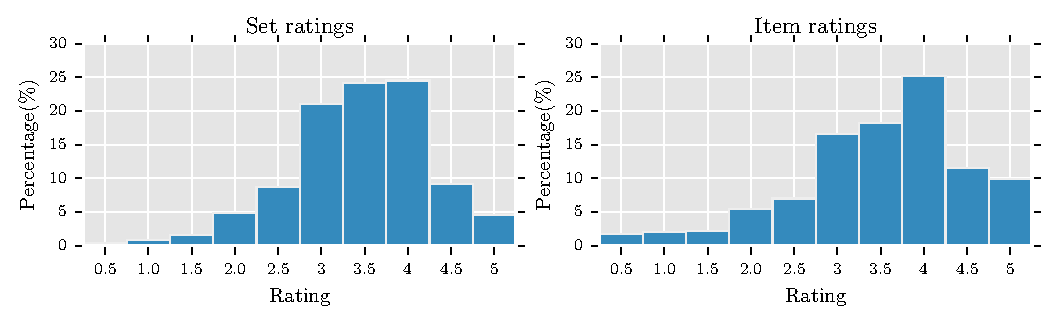
\includegraphics[scale=0.82]{figures/itemsetrating_horiz.pdf}}
  \caption{The distribution of the provided set ratings (left) and the ratings of
  their constituent items (right).}
  \label{fig:itemsetratingdist}
\end{figure}


In order to analyze how consistent a user's rating on a set is with the ratings provided by
the user on the movies in the set, 
we computed the difference of the average of the user's  ratings on the items in the set
and the rating assigned by a user to the set. We
will refer to this difference as \emph{mean rating difference} (MRD). 
Figure~\ref{fig:fractiondiversitymonths} (left) shows the distribution of the MRD values in
our datasets. The majority of the sets have
an MRD within a margin of 0.5 indicating that the users have rated them close to the
average of their ratings on set's items. The remaining of the sets have been
rated either significantly lower or higher from the average rating. We refer 
to these sets as the under- and
the over-rated sets, respectively. Moreover, an interesting observation from the
results in Figure~\ref{fig:fractiondiversitymonths} (right), is that the number of
under-rated sets is more than that of the over-rated sets. 


\begin{figure}[tb]
  \centerline{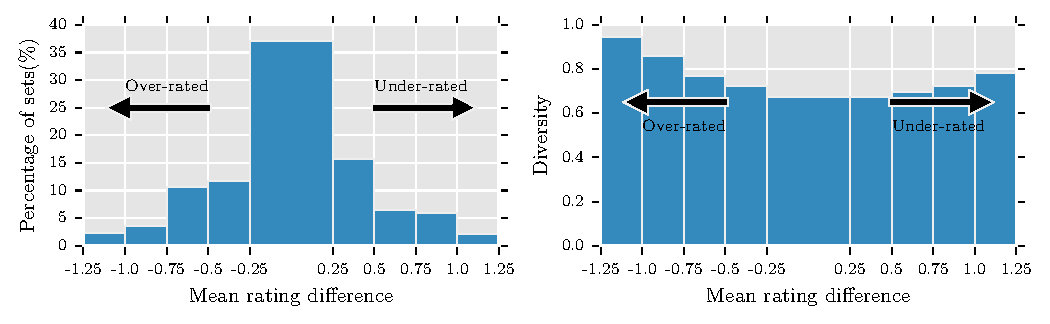
\includegraphics[scale=0.82]{figures/fractiondiversitymonths_exp_horiz.pdf}}
  \caption{Histogram of percentage of sets (left) and diversity (right) against
  mean rating difference (MRD).}
  \label{fig:fractiondiversitymonths}
\end{figure}


\begin{figure}[bt]
  \centerline{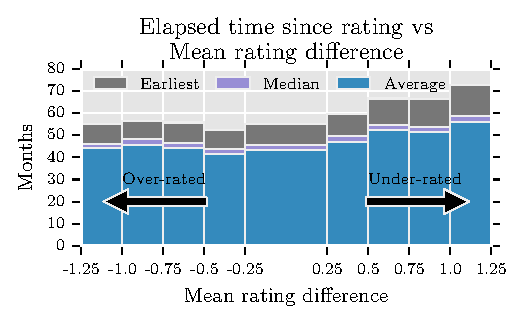
\includegraphics{figures/months_exp.pdf}}
  \caption{Histogram of elapsed time in months against mean rating difference.}
  \label{fig:elapsedmonths}
\end{figure}


\begin{figure*}[tb]
  \centerline{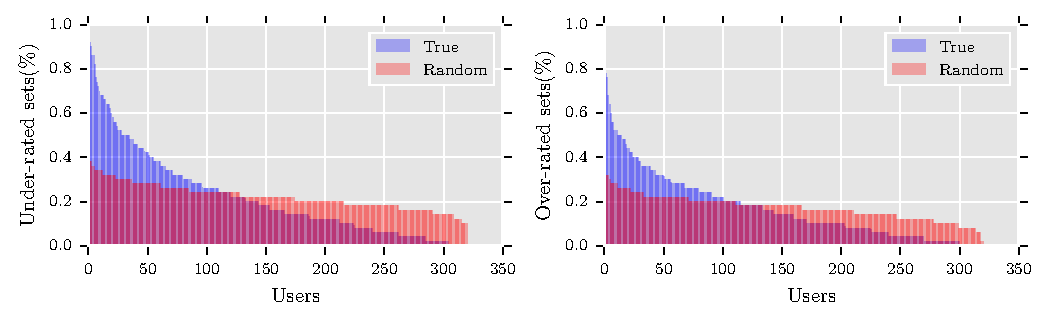
\includegraphics[scale=0.82]{figures/underoverrated_exp.pdf}}
  \caption{Fraction of under-rated and over-rated sets across users in true and
  random population.}
  \label{fig:underrated}
\end{figure*}

In order to understand what can lead to a set being under-
or over-rated, we investigated if the \emph{diversity} of the ratings of the
individual movies in a set could lead a user to under- or over-rate the set.
We measured the diversity of a set as the standard deviation of the ratings
that a user has provided to the individual items of the set.
As shown in Figure~\ref{fig:fractiondiversitymonths} (right), the sets 
that contain more diverse ratings (i.e., higher standard deviations) tend
to get under- or over-rated more often when compared to less diverse sets. This
trend was found to be
statistically significant ($p$-value of 0.01 using $t$-test).


Furthermore, we investigated whether the recently rated items
carry more weight than the items rated a long time ago. To this end, we computed
the difference between the timestamp of the earliest rating of the movies in the
set and the year 2016, i.e., when the users were asked to rate the sets.
Similarly, we computed the median and average age of movies in a set.
Interestingly as shown in Figure~\ref{fig:elapsedmonths}, the under-rated sets
contained movies whose ratings were provided on average five
years before the survey while the remaining sets contained the movies whose
ratings were provided on average four years before the survey. This difference
among the sets was found to be statistically significant ($p$-value $<$ 1e-16
using $t$-test). 
This suggests that the user's preference for a movie rated in the past carries
lower weight than the recently rated movie. 
The user's higher preference for a recent movie is not surprising as it has been
shown that the user tends to rate a movie close to the middle of the scale as
the time between viewing a movie and rating it increases~\cite{bollen2012remembering}.


Additionally, we studied if there are users that tend to consistently under- or
over-rate sets. To this end, we selected users who have rated at
least 50 sets and computed the fraction of their under- and over-rated sets.
We also computed the fraction of under- and over-rated sets across a random
population of the same size. We generated this random population by randomly
permuting the under-rated and over-rated sets across the users.
Figure~\ref{fig:underrated} shows the fraction of under- and over-rated sets
for both the true and random population of user. 
In the true population, some users tend to under- or over-rate sets
significantly more than that of the random population. Using the Kolmogorov-Smirnov 2 sample test, 
we found this behavior of true population to be statistically different ($p$-value $<$ 1e-16) from that of 
random population. 

The above analysis reveals that our dataset contains users that when they are
asked to assign a single rating to a set of
items, some of them consistently assign a rating that is lower than the
average of the ratings that they provided
to the set's constituent items (they under-rate), whereas others assign a rating
that is higher (they over-rate). Thus some
users are very demanding (or picky) and tend to focus on the worst items in the set,
whereas other users are less demanding and
tend to focus on the best items in the set. 


